\documentclass[a2paper, 12pt]{article}
\usepackage[font={huge, bf}]{caption}
\usepackage{fontspec}
\setmainfont{Arial}
\usepackage{subcaption}
\usepackage{graphicx}
\usepackage{tikz}
\usepackage{tikzsymbols}
\usetikzlibrary{calc,patterns,shapes.geometric}
\usepackage{float}
\usepackage{pdflscape}
\usepackage{geometry}
\geometry{landscape, margin=2cm}
\captionsetup[subfigure]{justification=justified,singlelinecheck=false}
\pagestyle{empty}

\def\centerarc[#1](#2)(#3:#4:#5){\draw[#1] ($(#2)+({#5*cos(#3)},{#5*sin(#3)})$) arc (#3:#4:#5);}

\begin{document}
	\vspace*{\fill}
	\begin{figure}[!htbp]
		\centering
		\begin{subfigure}[b]{0.48\textwidth}
			\caption{Figure 1}
			\centering
			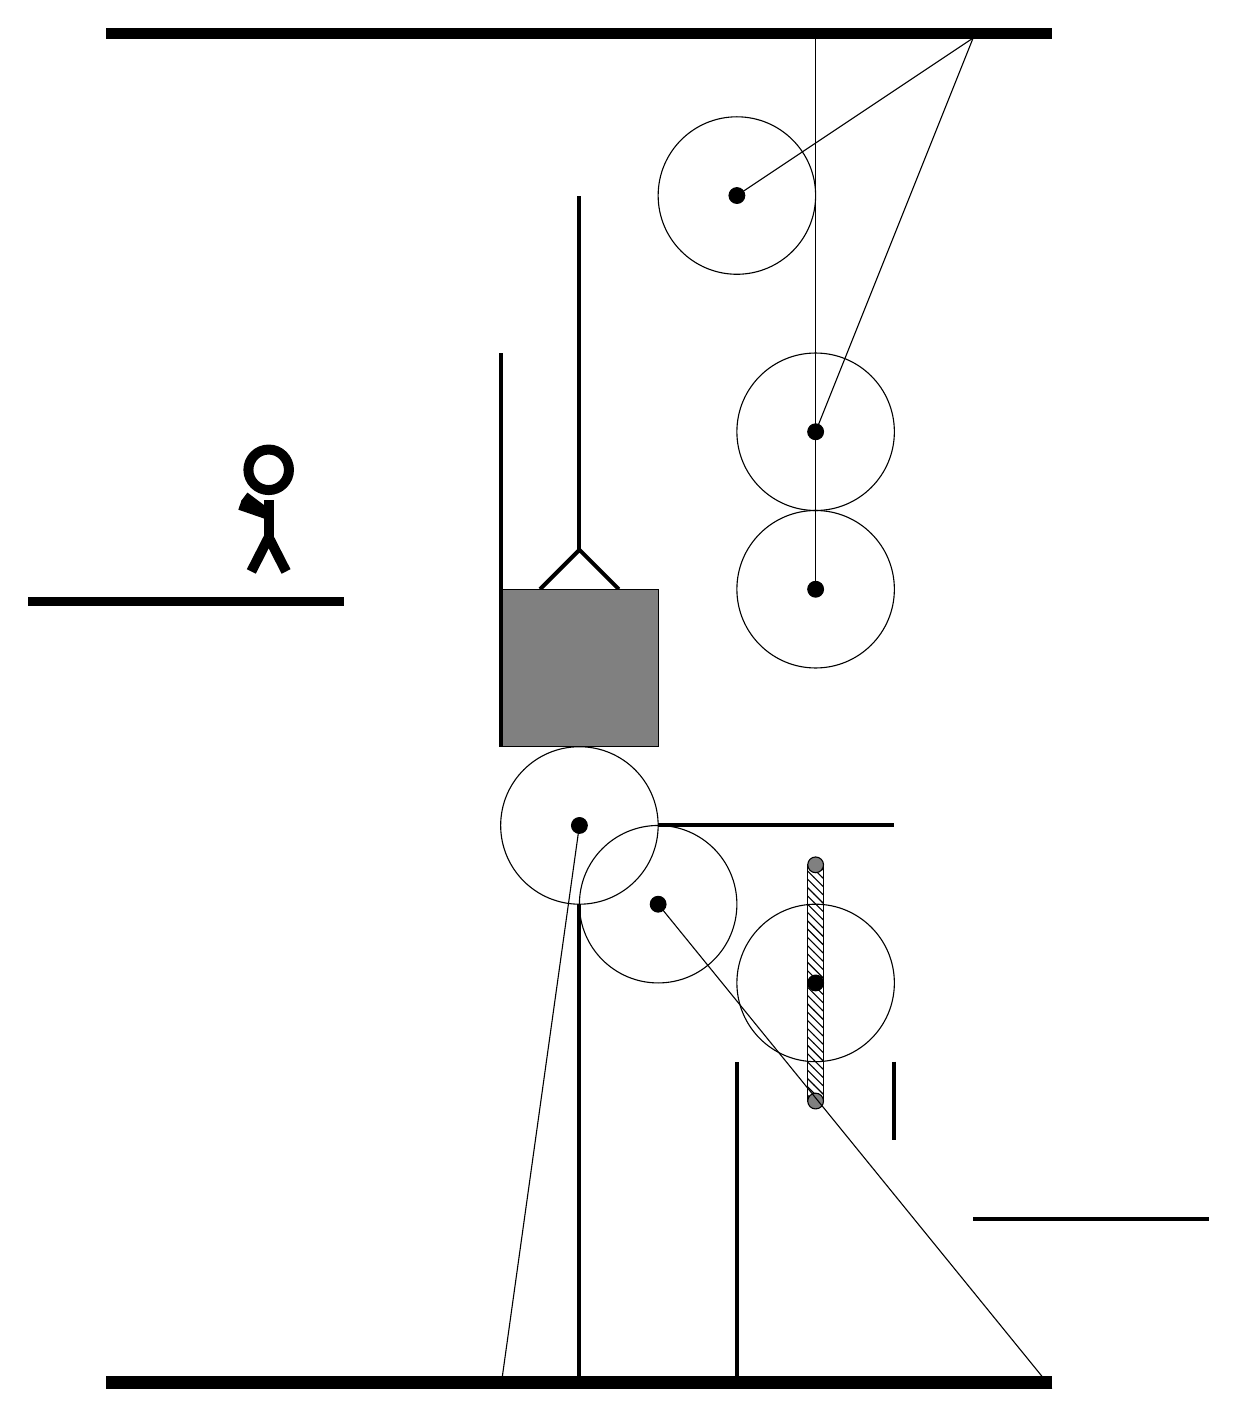
\begin{tikzpicture}
				\draw[fill=black] (-2, 14) rectangle (10, 14.125);
				
				\draw (7,7) circle (1);
				\draw[fill=black] (7,7) circle (0.1);
				\draw (7,14.0) -- (7,7);
				
				\draw (7,9) circle (1);
				\draw[fill=black] (7,9) circle (0.1);
				\draw (9,14.0) -- (7,9);
				
				\draw (6,12) circle (1);
				\draw[fill=black] (6,12) circle (0.1);
				\draw (9,14.0) -- (6,12);
				
				\draw (7,2) circle (1);
				\draw[fill=black] (7,2) circle (0.1);
				\draw[pattern=north west lines, pattern color=black] (6.9,3.5) rectangle (7.1,0.5);
				\draw[fill=black!50] (7,3.5) circle (0.1);
				\draw[fill=black!50] (7,0.5) circle (0.1);
				
				\draw (4,4) circle (1);
				\draw[fill=black] (4,4) circle (0.1);
				\draw (3,-3.15) -- (4,4);
				
				\draw (5,3) circle (1);
				\draw[fill=black] (5,3) circle (0.1);
				\draw (10,-3.15) -- (5,3);
				
				\draw[line width=0.5mm](4,7.5) -- (4,12.0);
				\draw[line width=0.5mm](3.5,7) --  (4,7.5) -- (4.5,7);
				\draw[fill=black!50] (3, 7) rectangle (5, 5);
				
				\draw[line width = 0.5mm] (5,4) -- (8,4);
				\centerarc[line width = 0.5mm](5,3)(90:180:1);
				\draw[line width = 0.5mm] (4,3) -- (4,-3);
				\centerarc[line width = 0.5mm](5,-3)(180:360:1);
				\draw[line width = 0.5mm] (6,-3) -- (6,1);
				\centerarc[line width = 0.5mm](7,1)(0:180:1);
				\draw[line width = 0.5mm] (8,1) -- (8,0);
				\centerarc[line width = 0.5mm](9,0)(180:270:1);
				\draw[line width = 0.5mm] (9,-1) -- (12,-1);
				\draw[line width = 0.5mm] (3,5) -- (3,10);
				
				\node at (0, 8) {\scriptsize \Strichmaxerl[10][-37][161]};
				\draw[fill=black] (-3, 6.9) rectangle (1, 6.8);
				
				\draw[fill=black] (-2, -3) rectangle (10, -3.15);
			\end{tikzpicture}
		\end{subfigure}
		\hfill
		\begin{subfigure}[b]{0.48\textwidth}
			\caption{Figure 2}
			\centering
			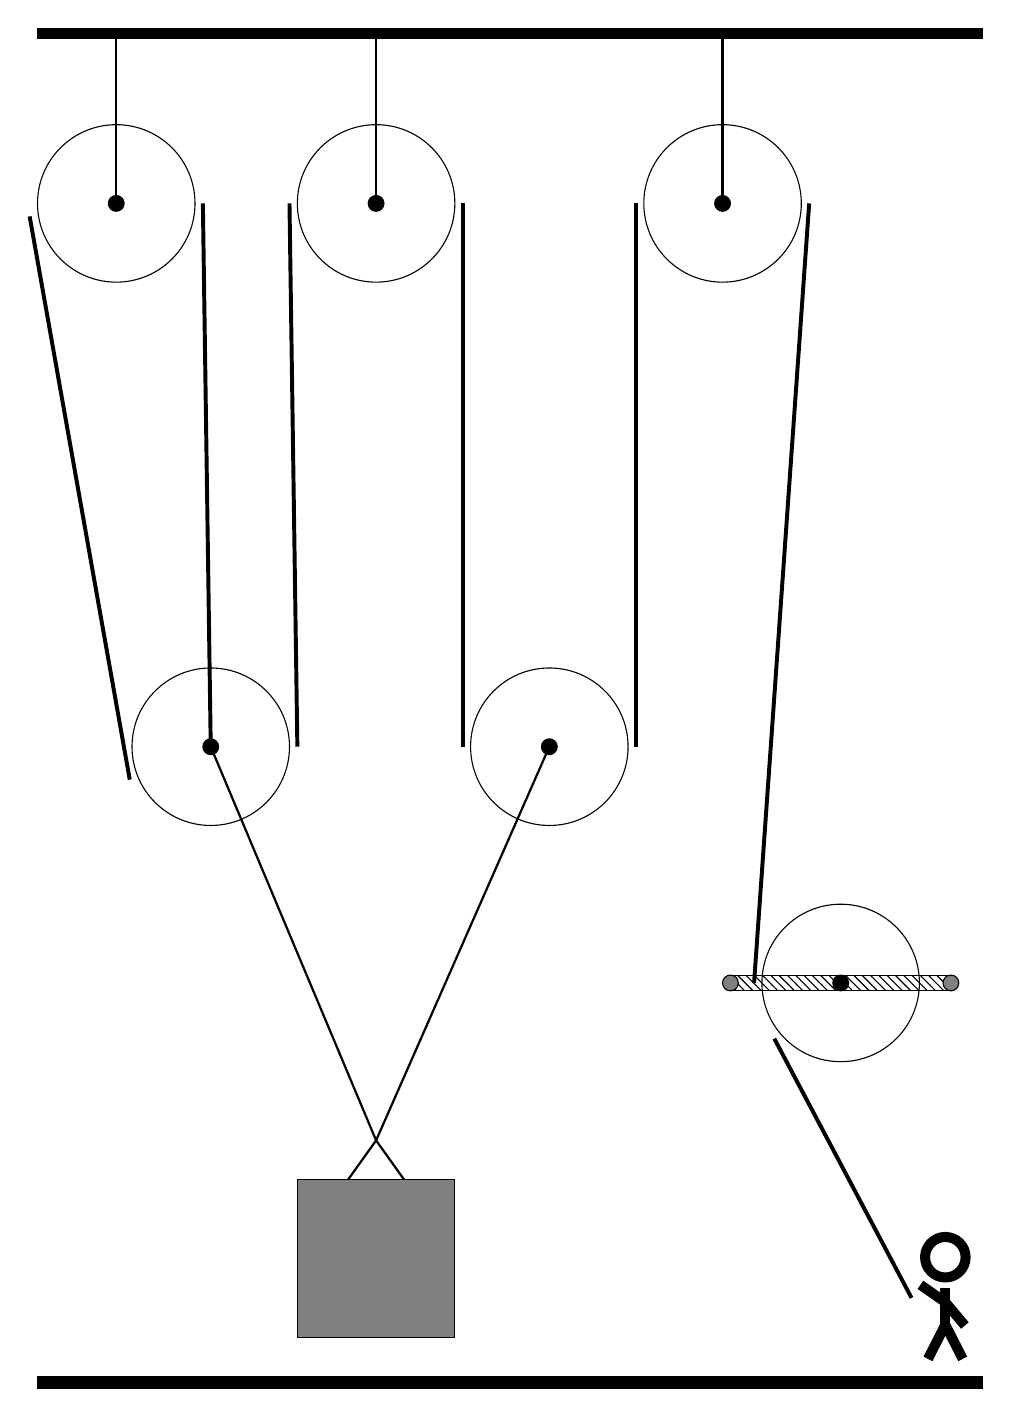
\begin{tikzpicture}
				\draw[fill=black] (-2, 14) rectangle (10, 14.125);
				
				\draw (-1, 11.9) circle (1);
				\draw[fill=black] (-1, 11.9) circle (0.1);
				\draw[thick] (-1, 11.9) -- (-1, 14);
				
				\draw (2.3, 11.9) circle (1);
				\draw[fill=black] (2.3, 11.9) circle (0.1);
				\draw[thick] (2.3, 11.9) -- (2.3, 14);
				
				\draw (6.7, 11.9) circle (1);
				\draw[fill=black] (6.7, 11.9) circle (0.1);
				\draw[thick] (6.7, 11.9) -- (6.7, 14);
				
				\draw (0.2, 5) circle (1);
				\draw[fill=black] (0.2, 5) circle (0.1);
				
				\draw (4.5, 5) circle (1);
				\draw[fill=black] (4.5, 5) circle (0.1);
				
				\draw (8.2, 2) circle (1);
				\draw[fill=black] (8.2, 2) circle (0.1);
				\draw[pattern=north west lines, pattern color=black] (6.8, 2.1) rectangle (9.6, 1.9);
				\draw[fill=black!50] (6.8, 2) circle (0.1);
				\draw[fill=black!50] (9.6, 2) circle (0.1);
				
				\draw[thick] (0.2, 5) -- (2.3, 0)  -- (4.5, 5);
				\draw[thick]  (1.8, -0.7) -- (2.3, 0) -- (2.8, -0.7);
				\draw[fill=black!50] (1.3, -0.5) rectangle (3.3, -2.5);
				
				\draw[line width=0.5mm] (0.2, 5) -- (0.1, 11.9);
				\centerarc[line width=0.5mm](-1, 11.9)(0:200:1.1);
				\draw[line width=0.5mm] (-2.1, 11.735) -- (-0.8285, 4.582);
				\centerarc[line width=0.5mm](0.2, 5)(200:360:1.1);
				\draw[line width=0.5mm](1.3, 5) -- (1.2, 11.9);
				\centerarc[line width=0.5mm](2.3, 11.9)(0:180:1.1);
				\draw[line width=0.5mm] (3.4, 11.9) -- (3.4, 5);
				\centerarc[line width=0.5mm](4.5, 5)(180:360:1.1);
				\draw[line width=0.5mm] (5.6, 5) -- (5.6, 11.9);
				\centerarc[line width=0.5mm](6.7, 11.9)(0:180:1.1);
				\draw[line width=0.5mm](7.8, 11.9) --  (7.1, 2);
				\centerarc[line width=0.5mm](8.2, 2)(180:220:1.1);
				\draw[line width=0.5mm](7.3574, 1.2929) -- (9.1, -2);
				
				\node at (9.5, -2) {\scriptsize \Strichmaxerl[10][-35][-50]};
				
				\draw[fill=black] (-2, -3) rectangle (10, -3.15);
			\end{tikzpicture}
		\end{subfigure}
	\end{figure}
		\vspace*{\fill}
\end{document}